\documentclass{sdqbeamer}
\titleimage{banner_2020_kit}
\groupname{Modelling for Continuous Software Engineering}

\title{Generierung von UML-Diagrammen aus PCM-Modellen}
\subtitle{Praktikum: Werkzeuge für agile Modellierung WS 2021/22}
\author{Sonya Voneva}

\date[21.03.22]{21. März 2022}

\begin{document}
\KITtitleframe

\begin{frame}{Inhaltsverzeichnis}
\tableofcontents
\end{frame}

\section{Motivation}
\begin{frame}{Motivation}
warum Visualisierung im Allgemeinen wichtig ist ...
\end{frame}

\begin{frame}[plain]
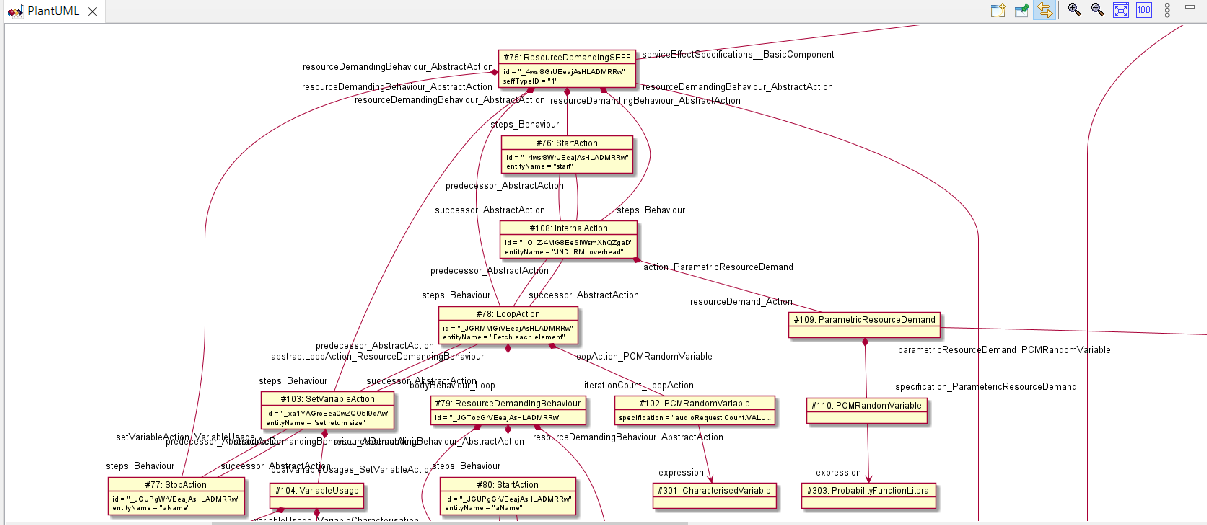
\includegraphics[width=\textwidth,height=1.1\textheight]{motivation.png}
\end{frame}

\section{Grundlagen}
\subsection{Palladio}
\begin{frame}{Palladio Framework}
\begin{columns}
\column{.3\textwidth}
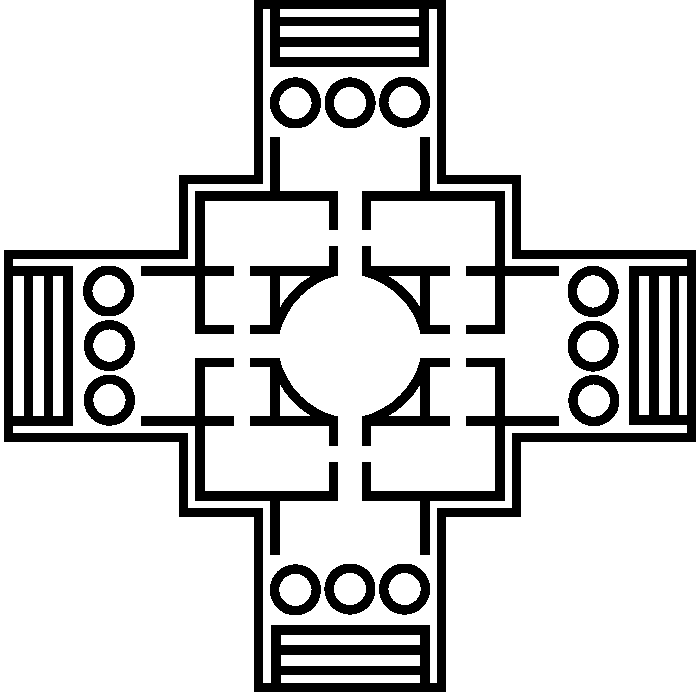
\includegraphics[width=\textwidth]{palladio.pdf}
\column{.7\textwidth}
\begin{itemize}
\item ...
\item .
\item ..
\end{itemize}
\end{columns}
\end{frame}
\begin{frame}
\centering
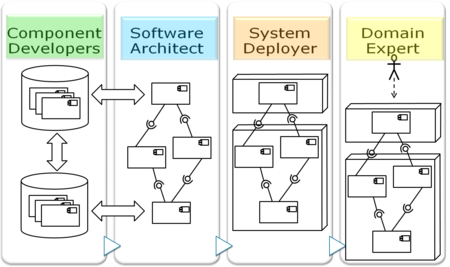
\includegraphics[width=.8\textwidth]{palladio_sichten.png}
\end{frame}
\subsection{PlantUML}
\begin{frame}{PlantUML}
\begin{columns}
\column{.7\textwidth}
\begin{itemize}
\item Erstellen von UML Diagrammen durch textuelle Notation
\item ein kurzes Beispiel?
\item ...
\end{itemize}
\column{.3\textwidth}
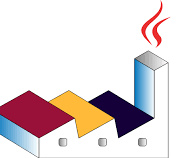
\includegraphics[width=\textwidth]{plantuml.jpg}
\end{columns}
\end{frame}

\section{Transformationen}
\subsection{Ansatz}
\begin{frame}{Ansatz}
\begin{enumerate}
\item Eigenes Bundle erstellen
\item Eigene Klasse für jeden Diagrammtyp
\item Durch die Palladio-Elemente iterieren -> in die textuelle PlantUML Notation "übersetzen"
\item Hyperlinks (z.B zu Repository) hinzufügen
\end{enumerate}
\end{frame}

\subsection{Architektur}
\begin{frame}{Architektur}
auf einem Diagramm den Erweiterungspunkt zeigen
\end{frame}

\subsection{PlantUML Diagramme}
\begin{frame}{Repository-Diagramm}
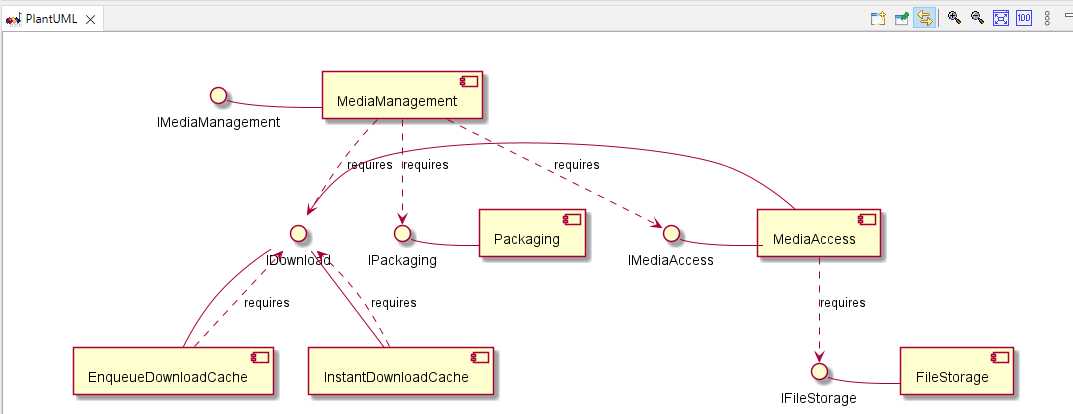
\includegraphics[width=\textwidth]{repository.png}
\end{frame}
\begin{frame}{Systemdiagramm}
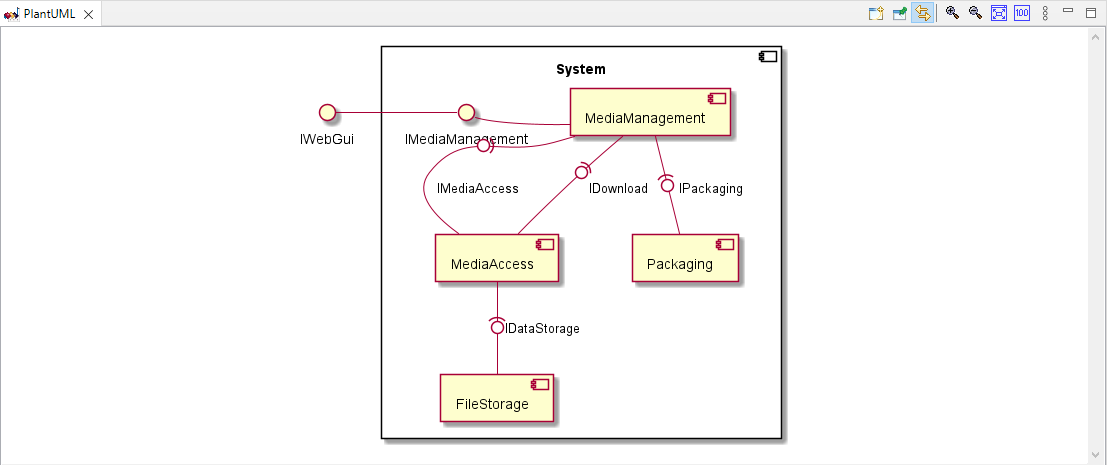
\includegraphics[width=\textwidth]{system.png}
\end{frame}
\begin{frame}{Allocation-Diagramm}
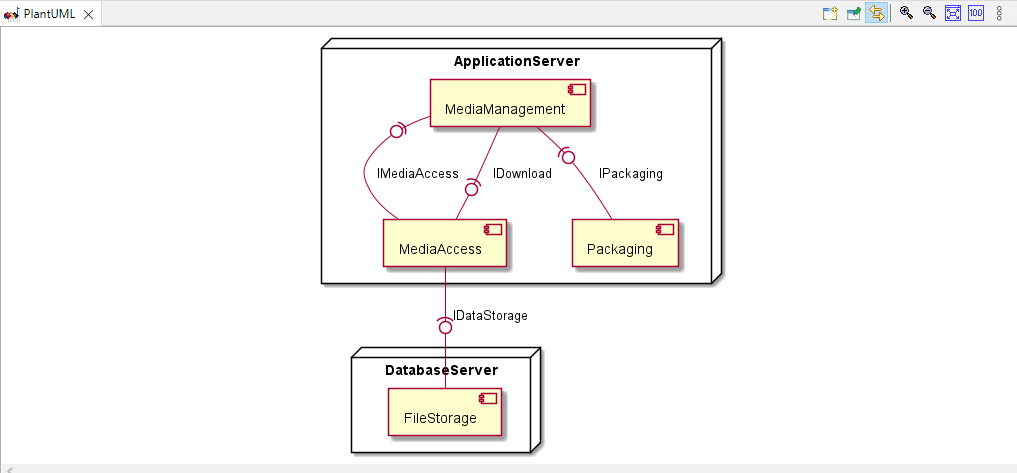
\includegraphics[width=\textwidth, height=.8\textheight]{allocation.png}
\end{frame}

\section{Einschränkungen}
\begin{frame}{Einschränkungen}
\begin{redblock}{eins}
= \texttt{}
\end{redblock}
\begin{redblock}{zwei}
= \texttt{}
\end{redblock}
\end{frame}

\section{Zusammenfassung}
\begin{frame}{Zusammenfassung}

\end{frame}

\end{document}
